% This is the preable, it must come before \begin{document}. 
% This is where you call all of the packages necessary to do cool stuff and define commands
\documentclass[12pt,titlepage]{article}
\usepackage{titling}
\usepackage{graphicx}
%\usepackage{geometry}  % for formatting margins
%\usepackage[margin=1.0in]{geometry} % to change the margins
\usepackage[bottom]{footmisc} % Forces footnotes to bottom of page
\interfootnotelinepenalty=10000 % Dont really know what this does, 
							   % stack exchange said it would make an error go away
\usepackage{fancyhdr}
\usepackage{float}      % So you can use the [H] for figures
\floatstyle{plaintop}   % These are something
\restylefloat{table}    % for tables, i guess
\usepackage{caption}
\usepackage{url}        % makes clickable urls
\urlstyle{rm}			% makes url fonts normal, not typewriter
\usepackage{hyperref}
\usepackage{amsmath,amssymb}
\usepackage{indentfirst}    % automatically indents first line of paragraph
\usepackage[super]{natbib}  % for bibliography
\usepackage [english]{babel} % For the next line so that the quote thing works
\usepackage [autostyle, english = american]{csquotes} % Fixes direction of quotation marks cus the quote button on Macs is dumb
\MakeOuterQuote{"}

\renewcommand{\thesection}{\Roman{section}.} 			% define section/subsection heirarcy, I like roman numerals
\renewcommand{\thesubsection}{\roman{subsection}.}
\renewcommand{\thesubsubsection}{\arabic{subsubsection}.} % end section/subsection heirarchy

\newcommand{\epnot}{\mbox{$\epsilon_{0}$}}
\newcommand{\mewnot}{\mbox{$\mu_{0}$}}
\providecommand{\e}[1]{\ensuremath{\times 10^{#1}}}		% exponent command
\usepackage{commath}
\def\mean#1{\left< #1 \right>}  % I make \mean{} will do this: <number>
\renewcommand\arraystretch{1.6} % SET TABLE ROW HEIGHT (MyValue=1.0 is for standard spacing)
\renewcommand*{\thefootnote}{\fnsymbol{footnote}} % make the footnote an asterisk instead of the default numbers


\begin{document}

%%%%%%%%%%%%%%%%%%%%%%%%%% Titlepage %%%%%%%%%%%%%%%%%%%%%%%%%%%%%%%%%%
\begin{titlepage}

\begin{minipage}{1in}
\begin{tabular}{l}
\end{tabular}
\end{minipage}
\hfill
\begin{minipage}{1in}
\begin{tabular}{r}
\end{tabular}
\end{minipage}


\begin{center}
% Upper part of the page

% Title
{ \huge \textbf{A Sample \LaTeX\; Lab Report} }\\[0.4cm]
\begin{center}
\vspace{2cm}
By\\
\large\textbf{Tyler Cohen}
\end{center}

%Affiliation
\begin{center}
\textit{\textmd{Department of Physics and Astronomy, Stony Brook University}}\\
\vspace{1cm}
\end{center}
\end{center}


\end{titlepage}


%%%%% BEGINNING OF REPORT %%%%%%

\begin{flushleft}
\section{Introduction and Theory}
\end{flushleft}
\par This is how you type text in \LaTeX, it's very simple. You can make your 
text \textbf{bold} or \textit{italicized} or \texttt{whatever this is}. The 
beauty of \LaTeX\: is in it's formatting. Look how easy it is to insert a 
footnote at the bottom of the page\footnote{This is a footnote.}.
%This is a comment. Comments are ignored by the compiler
\bigskip

\section{Methodology}
\par The main reason I will never go back to MS Word to write lab reports is 
because of the dumb-easy (and beautiful) way in which \LaTeX \: can format 
equations. Inline equations go in the math environment. Check it out: Gauss's 
Law is given by $\oint \vec{E} \cdot \vec{da} = \frac{Q_{enc}}{\epsilon_{0}}$ 
and states that the total electric flux out of any closed surface is proportional 
to the charge enclosed by the surface divided by the permittivity. It seems a 
little clunky at first, but you can't deny the elegance of typesetting a derivation:

\begin{eqnarray}
v_c &=& \frac{1}{C}\int{idt} \nonumber \\ \nonumber \\ % The \\ is a newline character and the \nonumber tells it not to number the equation, duh.
&=& \frac{I}{C}\int{sin(\omega t)dt} \nonumber\\ \nonumber \\ % The & are alignment characters, they keep the ='s lined up
&=& -\frac{I}{\omega C}cos(\omega t) \nonumber \\ \nonumber \\
&=& \frac{I}{\omega C}sin(\omega t - \frac{\pi}{2})	
\label{voltage_capacitor} %This is a label, it stores the argument to a variable and increments the equation counter
\end{eqnarray} 

You can label equations and refer to them later in the report like this 
\ref{voltage_capacitor}. This way, if you add another equation in before 
Equation (\ref{voltage_capacitor}), the \LaTeX \; compiler will update the 
number in the body of the text. (You have to compile twice for the number to be 
updated, the first time searches for labels and the second time passes the arguments.) 
Try to keep each line of your .tex source code under 80 characters. 
It improves code readability and makes it easier to debug.

\pagebreak
\section{Experimental}

\subsection{Data Acquisition}
\par This is how you make a table. Table (\ref{numbertable}) contains numbers.

\begin{center}  
\vspace{.3cm} % vertical space
\small{
\begin{tabular}{||c|c||} % set the number of columns, width, and delimeters on this line
\hline
\hline
Numbers & More Numbers \\
\hline
\hline
0.090 &	1.54 \\ \hline % mess with the hlines
0.502 &	9.98 \\ 
1.015 &	20.64 \\ \hline \hline
1.480 &	29.94 \\
1.997 &	40.55 \\ \hline \hline \hline
2.462 &	50.00 \\
2.950 &	60.36 \\
3.499 &	70.85 \\
3.823 &	80.22 \\
\hline
\end{tabular}}\\
\captionof{table}{\small \emph{These numbers were found with maths.}} 
\label{numbertable} 
\vspace{.4 cm}
\end{center}

\pagebreak
\subsection{Data Analysis}
\par It's also really easy to insert graphs and images in \LaTeX\; using the 
figure environment. \\

\begin{figure}[H] % An [h] tells LaTeX to put the image here. An [H] tells LaTeX PUT THE MU-FUCKIN IMAGE HERE!
\begin{center}
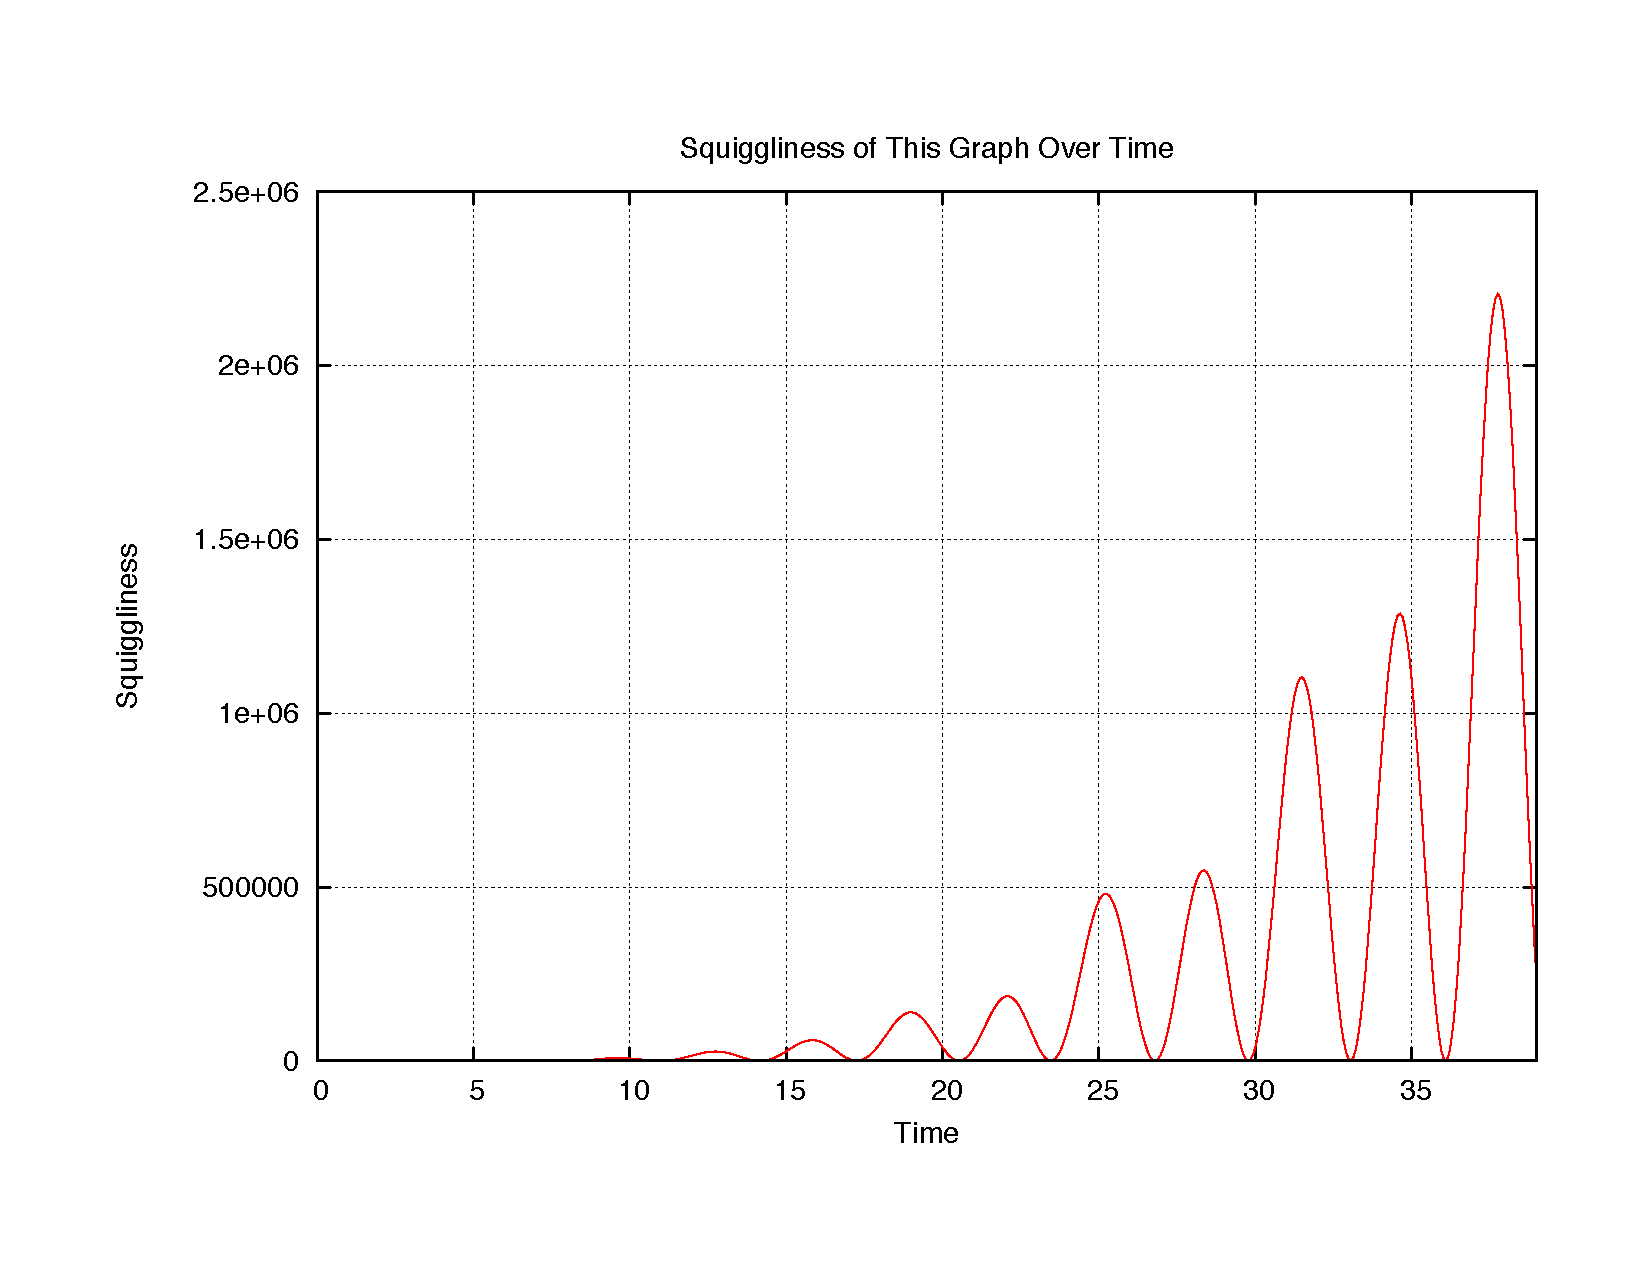
\includegraphics[scale=.55]{squiggliness.pdf} % If the file is not in the same directory as your .tex file you need to specify the absolute path
% Alternatively, using global parameters like \textwidth to define the size of the figure are better form
% E.g.
% 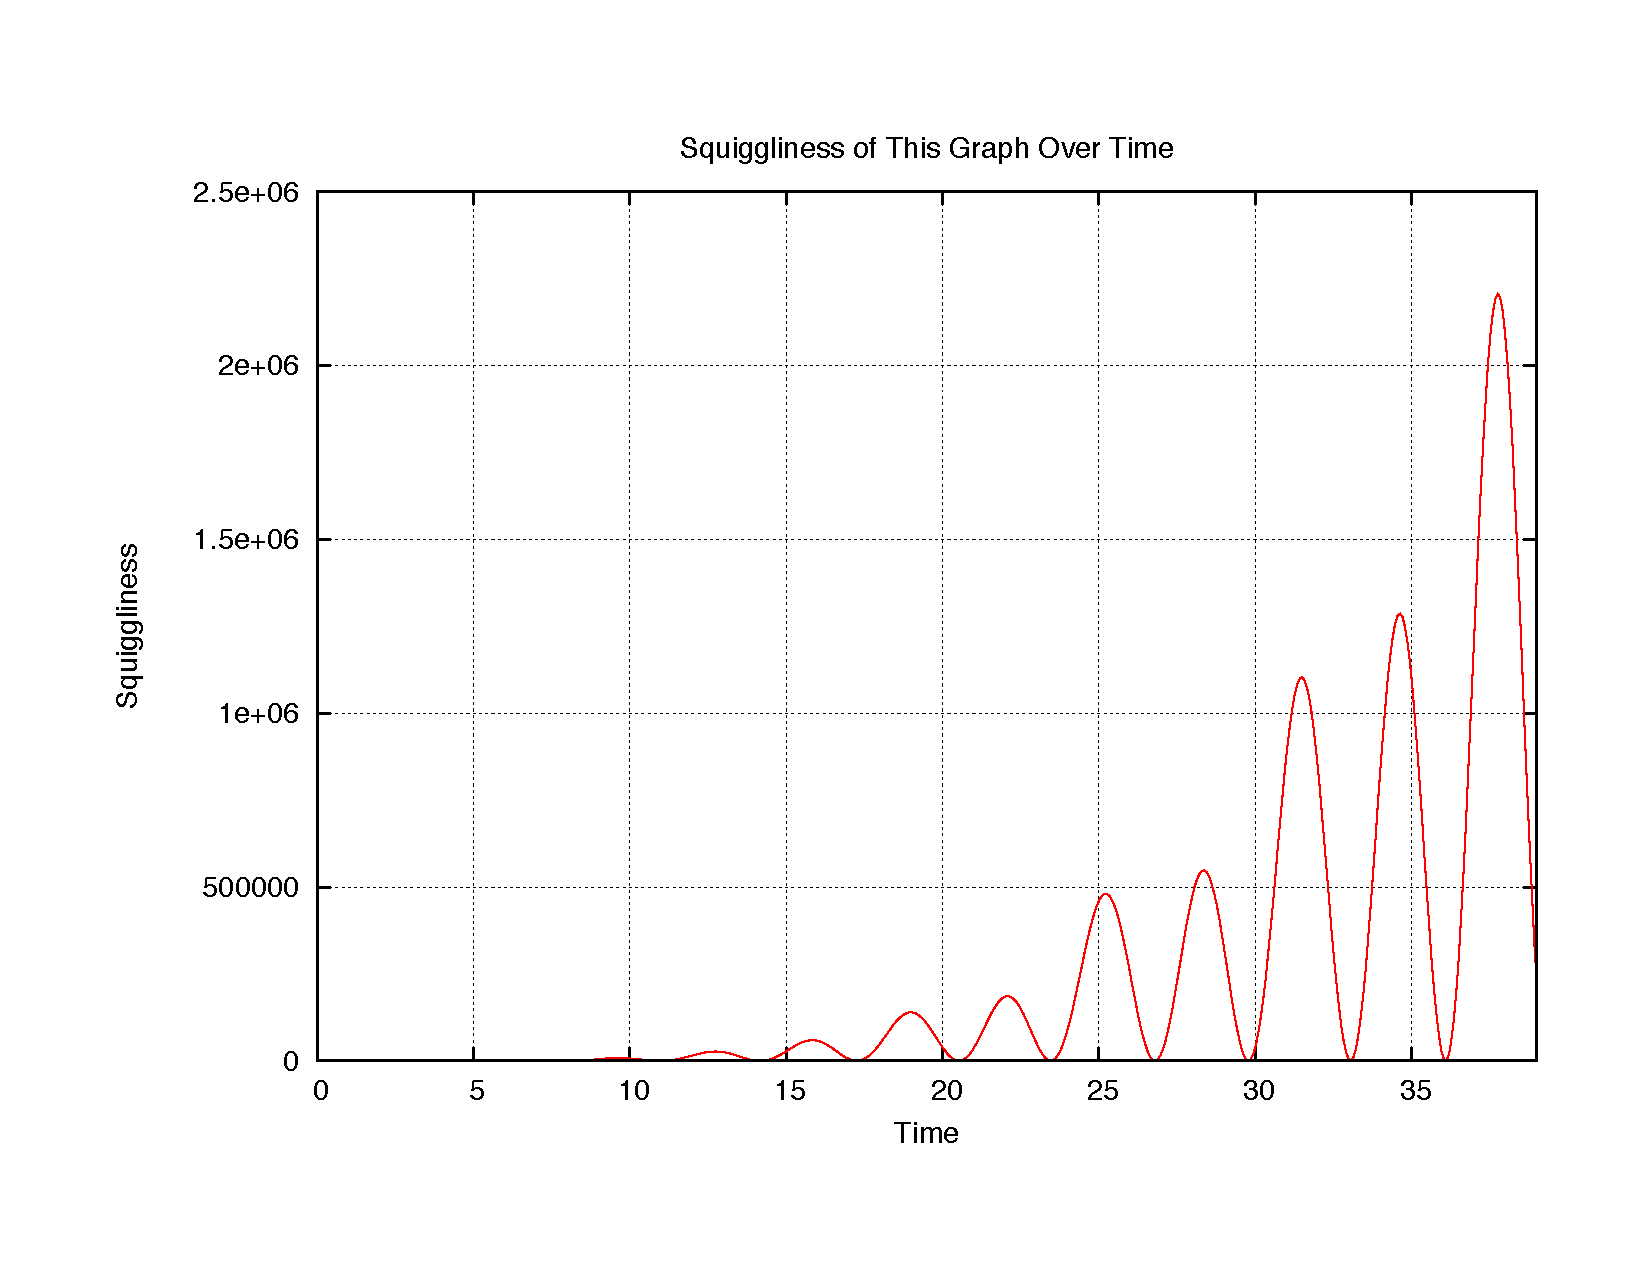
\includegraphics[width=0.9\textwidth]{squiggliness.pdf}
\caption{\small \emph{This graph is very squiggly}} 
\label{squiggly} %label arguments need to be the same as in \ref{}
\end{center}
\end{figure}

You can do the label thing with figures as well. We submit that the "squiggliness" 
of Fig (\ref{squiggly}) is related to the number of squiggles present in the graph.

\pagebreak
\section{Conclusion}
\par In conclusion, \LaTeX\; is awesome! This template does not even begin to 
cover a snowflake on the tip of the iceberg that is \LaTeX. The \url{Google}\cite{thegoogle} 
is your friend. If there's something you want to do in \LaTeX, chances are 
there's a package for it. Just try not to use too many packages or it will take 
forever to compile.


%%%%%%%%%%%%%%%%%%%%%%%%%%%%%%%% Bibliography %%%%%%%%%%%%%%%%%%%%%%%%%%%%%%%%
\newpage
\begin{thebibliography}{1}

\bibitem{thegoogle} \url{http://www.google.com}

\end{thebibliography}

\end{document}
